% Author: Paul Shao
% Email: paulshaoyuqiao1@berkeley.edu
\graphicspath{ {./} }
\qns{Warning! High Resistivity Zone Ahead!}

Resistivity is a physical property that quantifies how much the material opposes the flow of electric current.

Assume that in an ideal case, the cross-section and physical composition of the wire are uniform, We can find its resistivity with the equation below:

$$\rho = R \frac{A}{l}$$

Here, $\rho$ stands for the resistivity of the wire, $R$ stands for its resistance, $A$ stands for the area of the cross section of the wire, and $l$ stands for the length of the wire. Using this equation, we can also solve for the resistance of a wire:

$$R = \rho \frac{l}{A}$$
\sol{When you are showing this question to the students, make sure you present the resistor configuration from the perspective of circuit design. The purpose of this question is not to simply review equivalent resistance, but also to come up with a way to optimize a certain goal during the process of schematics design.}
\begin{enumerate}
    \item Now, consider the rectangular copper wire below. Given that the cross-section of the wire is a square and has a cross section area of $A$, determine the overall resistance of the wire in terms of $\rho_{cu}$, $L$, and $A$.
    \ans{By the resistivity equation, the resistance of the wire is equal to:
    $$R = \rho_{cu}\frac{L}{A}$$
    }
    \begin{center}
            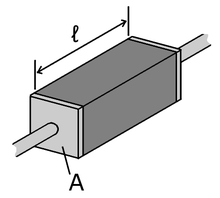
\includegraphics[scale=0.6]{../../questionBank/week05/q_resistivity_figs/wire.png}
    \end{center}
    \item Suppose we have $N$ such wires and align them side by side to form a mega-wire in the following fashion. Find the overall resistance of this mega-wire. What is this configuration similar to? \\
    \sol{When explaining this question to your students, make sure to show them a visual representation of the model. When drawing out the mega-wire, make sure to label the dimensions of the wire (cross-section area, length). It really helps to think visually in terms of how all the quantities that determine the resistance change.} \\
    \ans{Since we have all $N$ wires aligned side by side, we are essentially expanding the cross-section area while merging all the wires together by their lengths. This means that the new mega-wire will have a new cross-section area of $NA$ (since we are merging $N$ such wires), while its length remains the same ($L$). Hence, the overall resistance of the mega-wire will be:
    $$R_{mega} = \rho_{cu} \frac{L}{NA}$$
    }
    \item Again, with $N$ identical wires, what's a configuration that can achieve the highest resistance possible? What is this configuration similar to? \\
    \sol{The question by itself might seem pretty daunting and wide in scope. However, make sure you emphasize to the students to start by applying a circuit that they are familiar with (using equivalence). The proof that the series configuration achieves the highest resistance possible shouldn't be the main focus of this question. Although providing a intuitive explanation will help the students understand the approach more.}
    \ans{The key of this question is to start from the resistance equation:
    $$R = \rho\frac{l}{A}$$
    Algebraically, we want to maximize the value of $R$ for this question. Since $\rho$ is just a physical constant, we can't really manipulate its value. Observing the fraction $\frac{l}{A}$, we can see that the overall length of the mega-wire should be as great as possible, while its cross section area should be kept as small as possible. How can we arrange $N$ wires in a way so that the overall new wire is as long as possible? \\
    We arrange in a single long line! This also helps minimize the cross section area to $A$, and we can't really go lower than that since we can't split up a wire into two (thereby splitting the cross section area). \\
    Hence, for this new mega-wire, it has a length of $NL$ and a cross section area of $A$. Applying the resistance equation, we have:
    $$R_{mega} = \rho_{cu}\frac{NL}{A}$$
    This configuration is exactly the same as a series circuit where resistors are connected in one long line. If you think in terms of the equivalent resistance for a series circuit, it also makes sense since we are summing up all the resistances.
    }
    \item Consider part (b) again, but this time, instead of $N$ copper wires, we split the number evenly between aluminum wires and copper wires, and we again align them side by side to form a mega-wire (with the left half all aluminum , and right half all copper). What's the overall resistance of this wire? (In terms of $\rho_{cu}, \rho_{Al}, L, $ and $a$) \\
    \sol{Similar to the question above, this question also emphasizes thinking from the equivalent resistance perspective. Make sure to encourage your students to think in terms of the bigger picture (overall resistance) instead of individual wires. } \\
    \ans{As we can see from part (b), when we are aligning the wires side by side, we are essentially arranging the wires to be parallel to each other. Instead of thinking in terms of individual wires, we can consider the overall mega-wire to be a mega copper wire and a mega aluminum wire in parallel! For both wires, they will have a length of $L$ and an overall cross section area of $(N/2)A$ (since we have $N/2$ wires for each category). Hence, applying the resistance equation again, we can find that:
    $$R_{cu-mega} = \rho_{cu}\frac{L}{\frac{N}{2}A} = \rho_{cu}\frac{2L}{NA}$$
    $$R_{Al-mega} = \rho_{Al}\frac{L}{\frac{N}{2}A} = \rho_{Al}\frac{2L}{NA}$$
    Now, since these 2 mega wires are parallel to each other, by equivalent resistance, we can find the overall resistance of the wire to be:
    $$R_{overall} = \frac{1}{\frac{1}{R_{cu-mega}} + \frac{1}{R_{Al-mega}}} =\left( \frac{\rho_{cu}\rho_{Al}}{\rho_{cu} + \rho_{Al}} \right)\frac{2L}{NA}$$
    If you look closely at the equation, you can actually see how the resistivities of both materials are arranged algebraically as if they are in parallel!
    }
    \item Instead of having all the $N/2$ copper wires on the right side, now all the wires are mixed together (a copper wire can be aligned right next to an aluminum wire), does the overall resistance of this new mega-wire change? \\
    \sol{This might seem like a tricky question because there are a lot of different ways to permute all the $N$ wires. However, the key point is still on the bigger picture. Make sure to encourage the student to think in terms of equivalence (not just equivalent resistance, but also how you can actually move things around in certain circuits!)} \\
    \ans{The key to this question is to realize that, we are essentially aligning all wires in parallel, so we can rearrange all the copper wires to be together on one side and all the aluminum wires to be together on another side, and now we are back to the previous question! Hence, the overall resistance of this new mega-wire doesn't change.}
\end{enumerate}
